\documentclass[a4paper, 14pt]{extarticle}%тип документа

\date{}

\usepackage{indentfirst}

\usepackage{graphicx}
\usepackage{cmap}
\usepackage[T2A]{fontenc}
\usepackage[utf8]{inputenc}

\usepackage{indentfirst}

%%\renewcommand{\footrulewidth}{ .0em }
\usepackage[english,russian]{babel}
\usepackage{multirow} % Слияние строк в таблице
\newcommand
{\un}[1]
{\ensuremath{\text{#1}}}


%Русский язык
\usepackage[T2A]{fontenc} %кодировка
\usepackage[utf8]{inputenc} %кодировка исходного кода
\usepackage[english,russian]{babel} %локализация и переносы

%Таблицы
\usepackage[table,xcdraw]{xcolor}
\usepackage{booktabs}

%Математика
\usepackage{amsmath, amsfonts, amssymb, amsthm, mathtools}

%отступы 
\usepackage[left=2cm,right=2cm,top=2cm,bottom=3cm,bindingoffset=0cm]{geometry}

%Вставка картинок
\usepackage{graphicx}
\usepackage{wrapfig, caption}
\graphicspath{}
\DeclareGraphicsExtensions{.pdf,.png,.jpg, .jpeg}
\newcommand\ECaption[1]{%
     \captionsetup{font=footnotesize}%
     \caption{#1}}

%Таблицы
\usepackage[table,xcdraw]{xcolor}
\usepackage{booktabs}

%Графики
\usepackage{pgfplots}
\pgfplotsset{compat=1.9}


\usepackage[english,russian]{babel}
\usepackage{multirow} % Слияние строк в таблице
\newcommand
{\un}[1]
{\ensuremath{\text{#1}}}

\begin{titlepage}
	\begin{center}
		\large 	Московский физико-технический университет \\
		Физтех-школа радиотехники и компьютерных технологий\\
		\vspace{0.2cm}
		
		\vspace{4.5cm}
		Лабораторная работа № 3.5.1 \\ \vspace{0.2cm}
		\LARGE \textbf{Изучение плазмы газового разряда в неоне}
	\end{center}
	\vspace{2.3cm} \large
	
	\begin{center}
		Работу выполнил: \\
		Шурыгин Антон \\
		Б01-909

	\end{center}
	
	\begin{center} \vspace{60mm}
		г. Долгопрудный \\
	\end{center}
\end{titlepage}

%Русский язык
\usepackage[T2A]{fontenc} %кодировка
\usepackage[utf8]{inputenc} %кодировка исходного кода
\usepackage[english,russian]{babel} %локализация и переносы

%отступы 
\usepackage[left=2cm,right=2cm,top=2cm,bottom=3cm,bindingoffset=0cm]{geometry}

%Вставка картинок
\usepackage{graphicx}
\usepackage{wrapfig, caption}
\graphicspath{}
\DeclareGraphicsExtensions{.pdf,.png,.jpg, .jpeg}
\newcommand\ECaption[1]{%
     \captionsetup{font=footnotesize}%
     \caption{#1}}



\begin{document}
\maketitle
\paragraph{Цель работы:}изучение вольт-амперной характеристики тлеющего разряда; изучение свойств плазмы методом зондовых характеристик.
\paragraph{В работе используются:} стеклянная газоразрядная трубка, наполненная неоном; высоковольтный источник питания, источник питания постоянного тока; делитель напряжения; потенциометр; амперметры; вольметры; переключатели. 

\section{Краткая теория}

Одним из самых простых методов исследования свойств плазмы является измерение электрических потенциалов с помощью зондов(небольших проводников, вводимых в плазму). В нашей работе используется двойной зонд. Его удобно использовать для нахождения различных параметров плазмы, таких как температура или концентрация частиц.

Рассчитаем величину тока, проходящего через двойной зонд вблизи точки $I=0$. 
Напряжение $U$ между зондами равно расзности потенциалов на первом и втором:
\begin{equation}
    U = U_{2}-U_{1}= (U_{f}+\Delta U_{2}) - (U_{f}+\Delta U_{1}) = \Delta U_{2} - \Delta U_{1}
\end{equation}

Найдем ток, приходящий на первый электрод:

   \[I_{1} = I_{in} - I_{e_0} \cdot exp{\frac{e U_{1}}{k_{B} T_{e}}} = I_{in} - \left[I_{e_0} \cdot exp{\frac{e U_{f}}{k_{B} T_{e}}} \right] \cdot exp{\frac{e \Delta U_{1}}{k_{B} T_{e}}} \]
   
   
При $\Delta U_{1} = 0$ электронный и ионный ток компенсируют друг друга. Поэтому множитель, заключенный в квадратные скобки равен $I_{iн}$. Поэтому

\begin{equation}
   I_{1} = I_{in} \left[1 - exp{\frac{e U_{1}}{k_{B}}} \right]
\end{equation}

Аналогично для $I_{2}$. Так как зонды соединены последовательно, то $I_{1} = -I_{2} = I$. Тогда выразим $U$ 

\[ U = \Delta U_{1} - \Delta U_{2} = \frac{k_{B} T_{e}}{e} ln{(1 - \frac{I}{I_{in}})} - \frac{k_{B} T_{e}}{e} ln{(1 + \frac{I}{I_{in}})}  = \frac{k_{B} T_{e}}{e} ln{\frac{I_{in} - I}{I_{in} + I}} \]

Разрешив относительно $I$, получим
\begin{equation}
   I_{1} = I_{in} th{\frac{e U}{2 k_{B} T_{e}}}
\end{equation}

Прдиффиренцировав по $U$ в точке $U = 0$, получим
\begin{equation}
   k_{B} T_{e} = \frac{1}{2} \frac{e I_{in}}{\frac{dI}{dU}}
\end{equation}

Здесь $\frac{dI}{dU}$ - наклон характеристики зонда вблизи начала координат, а  $ I_{in} $
\begin{equation}
I_{in} = 0,4 n_{i} e S \sqrt{\frac{2 k_{B} T_{e}}{m_{i}}}
\end{equation}

Плазменную частоту колебаний электронов можем рассчитать по формуле:
\begin{equation}
\omega_{p} = \sqrt{\frac{4 \pi n_{e} e^2}{m_{e}}} = 5,6 \cdot 10^4 \sqrt{n_{e} \text{см}^{-3}} \: \text{рад/сек}  
\end{equation}

Дебаевский радиус $R_{D}$, приняв $ T_{i} \approx  300 K $, рассчитаем из формулы:
\begin{equation}
r_{D} = \sqrt{\frac{k T_{i}}{4 \pi n_{i} e^2}} \: \text{см}
\end{equation}

Среднее число ионов в дебаевской сфере (должно быть $ N_{D} >> 1$):
\begin{equation}
N_{D} = n_{i} \frac{4}{3} \pi {r_{D}}^3
\end{equation}

Степень ионизации плазмы можно оценить как:
\begin{equation}
\alpha = \frac{n_{i}}{n}
\end{equation}

где $n$ находится из уровнения $P = n k T $ при $P \approx 1 \: \text{мбар}$ (при нормальных условиях $n= N_{L}$, $N_{L}$ - число Лошмидта).


\begin{figure}[h!]
\begin{center}
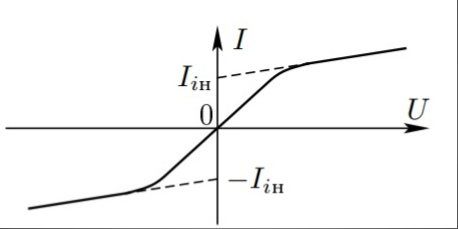
\includegraphics[width=0.7 \textwidth]{zalupa_vodolaza.jpg}
\end{center}
\ECaption{Вольт-амперная характеристика двойного зонда}
\end{figure}


Схема установки для исследования плазмы газового разряда в неоне представлена на рис.1

\begin{figure}[h!]
\begin{center}
\includegraphics[width=1 \textwidth]{pictures/lab351_pic1.png}
\end{center}
\ECaption{Схема  установки для исследования газового разряда}
\end{figure}

Стеклянная газоразрядная трубка имеет холодный полый катод, три анода, геттерный узел - стеклопоглощающая пленка. Трубка наполнена изотопом неона при давлении 2 мм. рт. ст.. Катод и один из анодов с помощью подключателя П1 подключаются через балластный резистор $R_b$ ($\approx 500 \: \text{кОм}$) к регулируемому высоковольтному ист. питания с вых. напряжением до нескольких киловольт.

При подключении к ВИП анода - 1 между ним и катодом возникает газовый разряд. Ток разряда имеряется милиамперметром $А1$, падению напряжения на трубке вольметром - $V1$, подключенным к трубке через высокоомный делитель напряжения с коэффциентом $\frac{R_1 + R_2}{R_1}$

При подключении к ВИП анода - 2 разряд возникает в пространстве между катодом и анодом - 2 , где нахожится двйоной зонд, используемый для диагностики плазмы положительного столба. 




\section{Выполнение работы}

Данные установки $R_b = $ 450 $\: kOm, d = $ 0.2 $\: mm, l =$  5.2 $\: mm$

 \subsection{Вольт-амперная характеристика разряда}

Снимаем значения, составляем таблицу 1:
                
\begin{table}[!]
    \caption{Таблица c измерениями}
        \begin{center}
            \begin{tabular}{| c | c | c | c |}
            \hline
            \textbf{V, volt} & \textbf{I, mkA} & \textbf{V, volt} & \textbf{I, mkA}\\
            \hline
            34.43 & 0.5 & 27.26 & 4.4\\
            \hline
            33.14 & 0.76 & 27.27 & 3.76\\
            \hline
            32.04 & 1.24 & 27.47 & 3.2\\
            \hline
            30.1 & 1.64 & 28.09 & 2.62\\
            \hline
            28.79 & 2.36 & 29.22 & 2.14\\
            \hline
            27.94 & 2.86 & 30.05 & 1.78\\
            \hline
            27.59 & 3.34 & 32.05 & 1.22\\
            \hline
            27.4 & 3.72 & 33.83 & 0.62\\
            \hline
            27.36 & 4 & -16.3 & -32.75\\
            \hline
            27.41 & 4.36 & -19.12 & -33.95\\
            \hline
            27.38 & 4.96 & -22.32 & -35.38\\
            \hline
            27.22 & 5 & -24.91 & -36.43\\
            \hline
            \end{tabular}
        \end{center}
    \label{A_table}
\end{table}

По полученным значениям строим график зависимости U(I) - вольт-амперную характеристику разряда. 

\begin{figure}[h!]
	\centering
	\includegraphics[width=1.1\linewidth]{pictures/lab351_0.jpg}
	\caption{График зондовой характеристик $i_{razr} = 5 \: mA$}
	\label{C}
\end{figure}

По наклону касательной к графику определим максимальное дифференциальное сопротивление разряда $R_{max} \approx 2 \: kOm \:$:

\subsection{Работа с зондом}

Погрешность при данных измерениях - погрешность амперметра тока разряда - $\sigma{I_{rarz}} = 0.03 \: mA$
Снимаем значения, составляем таблицу 2:


\begin{table}[!]
\caption{Таблица c измерениями}
    \begin{center}
        \begin{tabular}{| c | c | c | c | c | c |}
        \hline
        \textbf{U1, volt} & \textbf{I1m mkA} & \textbf{U2, volt} & \textbf{I2, mkA} & \textbf{U3, volt} & \textbf{I3, mkA} \\
        \hline
        24,91 & 24.89 &   24.91   & 90.91 & 24.91 & 52.54\\
        \hline
        21.36 & 23.94 & 21.33 & 91.09 & 21.79 & 50.64\\
        \hline
        18.86 & 23.31 & 18.27 & 89.2 & 18.03 & 48.38\\
        \hline
        15.37 & 22.38 & 14.59 & 84.05 & 14.92 & 46.37\\
        \hline
        11.85 & 20.93 & 10.5 & 71.16 & 12.31 & 43.62\\
        \hline
        8.76 & 17.79 & 9.14 & 64.39 & 9.76 & 38.86\\
        \hline
        7.27 & 15.28 & 8.3 & 59.41 & 6.17 & 26\\
        \hline
        6.23 & 13.09 & 7.49 & 53.87 & 5.36 & 21.92\\
        \hline
        5.26 & 10.62 & 7.65 & 55.04 & 4.26 & 15.8\\
        \hline
        4.26 & 7.88 & 6.69 & 48 & 2.69 & 6.12\\
        \hline
        3.53 & 5.62 & 5.36 & 36.81 & 2.04 & 1.81\\
        \hline
        2.44 & 1.83 & 4.13 & 25.11 & 1.78 & 0\\
        \hline
        1.94 & 0.16 & 1.78 & 0.41 & -0.78 & -15.4\\
        \hline
        -1.94 & -13.21 & -1.77 & -29.95 & -2.33 & -25.6\\
        \hline
        -3.29 & -17.49 & -3.55 & -47.48 & -3.46 & -32\\
        \hline
        -4.44 & -20.5 & -4.12 & -52.58 & -5.15 & -40.43\\
        \hline
        -5.56 & -23.08 & -5.04 & -60.34 & -7.17 & -48.21\\
        \hline
        -6.9 & -25.48 & -6.14 & -68.57 & -8.85 & -52.74\\
        \hline
        -8.01 & -27.04 & -7.32 & -76.24 & -10.95 & -56.71\\
        \hline
        -9.87 & -29.14 & -8.95 & -84.92 & -14.37 & -60.63\\
        \hline
        -10.7 & -29.81 & -10.13 & -90.05 & -18.12 & -63.58\\
        \hline
        -13.2 & -31.35 & -13.09 & -99.2 & -21.16 & -65.62\\
        \hline
        -16.3 & -32.75 & -15.95 & -104.67 & -23.36 & -67.18\\
        \hline
        -19.12 & -33.95 & -19.62 & -108.4 & -24.91 & -68.31\\
        \hline
        -22.32 & -35.38 & -21 & -109.22 &  & \\
        \hline
        -24.91 & -36.43 & -24.91 & -110.1 &  & \\
        \hline
  	\end{tabular}
  \end{center}
\label{A_table}
\end{table}

По полученным значениям строим графики зависимости $I(U)$:

\begin{figure}[h!]
	\centering
	\includegraphics[width=1.1\linewidth]{pictures/lab351_all.png}
	\caption{Графики I(U) для трех разл. токов разряда. Зондовые характеристики}
	\label{C}
\end{figure}

\begin{figure}[h!]
	\centering
	\includegraphics[width=1.1\linewidth]{pictures/lab351_1.5.png}
	\caption{График зондовой характеристик $i_{razr} = 1,5 \: mA$}
	\label{C}
\end{figure}


\begin{figure}[h!]
	\centering
	\includegraphics[width=1.1\linewidth]{pictures/lab351_3.png}
	\caption{График зондовой характеристик $i_{razr} = 3 \: mA$}
	\label{C}
\end{figure}

\begin{figure}[h!]
	\centering
	\includegraphics[width=1.1\linewidth]{pictures/lab351_5.png}
	\caption{График зондовой характеристик $i_{razr} = 5 \: mA$}
	\label{C}
\end{figure}


\newpage


По графикам 1, 2, 3, 4 рассчитаем $I_{насыщ}$, а так же $\frac{dI}{dU}, \: U = 0$.
Для этого проводим соответствующие ассимптоты и касательные. Сведем полученные результаты в таблицу 1:

	
\begin{table}[!]
  \caption{Таблица для расчетов}
  \begin{center}
  	\begin{tabular}{|c|c|c|}
  	    \hline
  `	$$I_{razr}, mA$$ & $I_{iH}, mkA$ & $\frac{dI}{dU}, \frac{mkA}{V}$ \\
  	    \hline
  	1.5 & 19 & 6.96  \\
  		\hline
  	3.0 & 39 & 32 \\
  		\hline
  	5.0 & 73 & 82  \\
  		\hline
  	\end{tabular}
  \end{center}
\label{B_table}
\end{table}


Учтем погрешности.

\textbf{Теперь рассчитаем температуру электронов} $T_e$ по формуле (?), а также $n_e$ - концентрацию электронов в плазме по формуле Бома (?).

\begin{table}[!]
  \caption{Таблица для расчетов}
  \begin{center}
  	\begin{tabular}{|c|c|c|c|c|}
  	    \hline
  	$ I_{razr}, \: mA $ & $ k T_e, \: el\cdot Volt $ & n_e \cdot $10^{15}, m^{-3}$ & T_e, K \cdot 10^{4} & \sigma{T_e}, \: K \cdot 10^{4} \\
  	    \hline
  	1.5 & 1.36 & 26.3 & 1.6 & 0.18 \\
  		\hline
  	3.0 & 0.64 & 44 & 0.7 & 0.08 \\
  		\hline
  	5.0 & 0.44 & 77 & 0.5 & 0.06 \\
  		\hline
  	\end{tabular}
  \end{center}
\label{B_table}
\end{table}

Построим график зависимости $ n_{e} = f(I_{razr})$

\begin{figure}[h!]
	\centering
	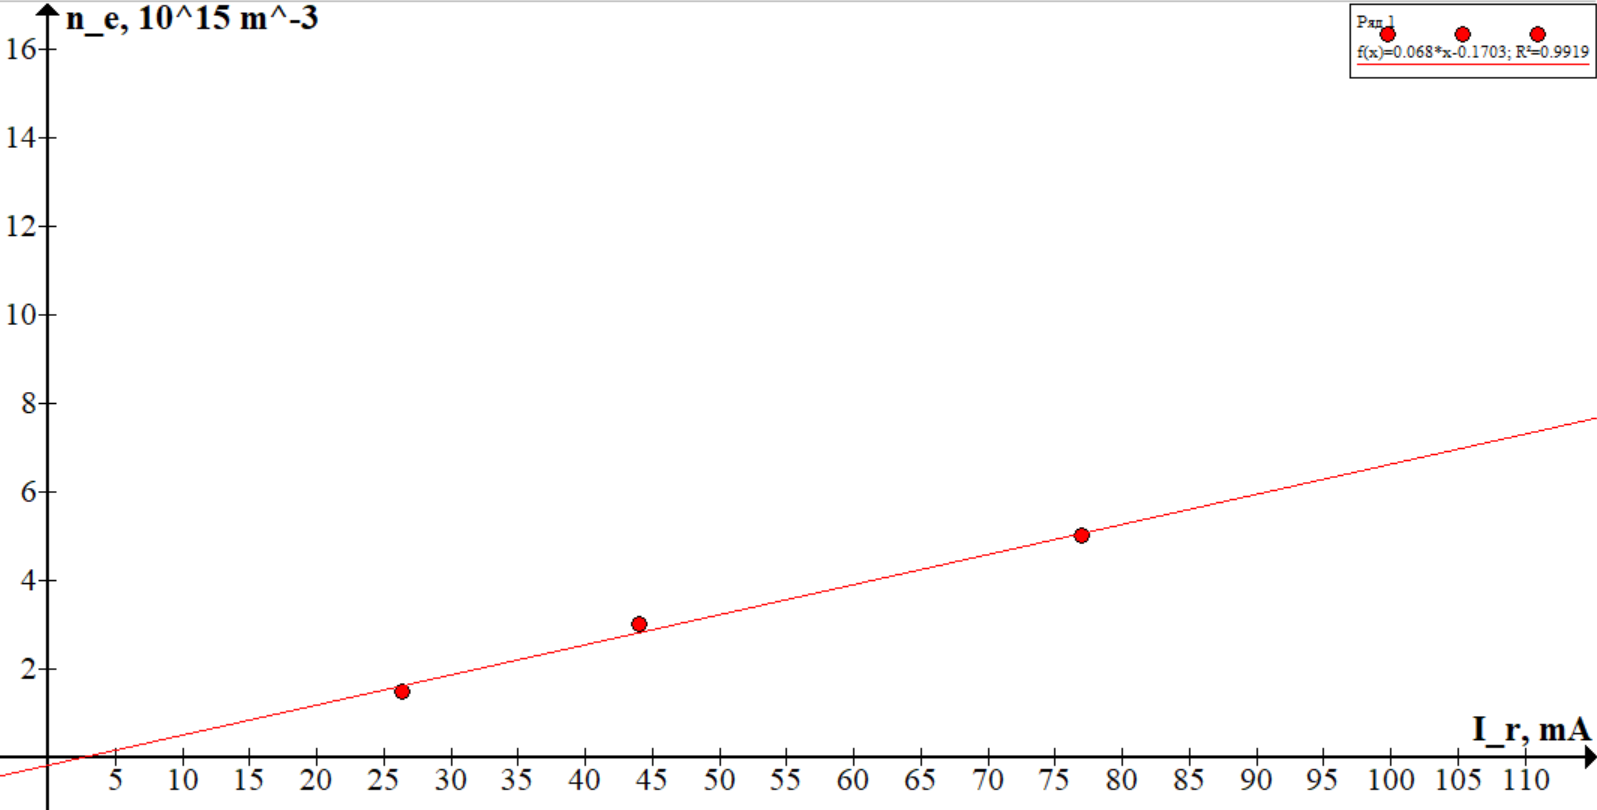
\includegraphics[width=1.1\linewidth]{пенис игоря.png}
	\caption{График зависимости n_{e} от I_{razr}}
	\label{C}
\end{figure}


\textbf{Затем рассчитаем плазменную частоту колебаний электронов} $\omega_e$, а так же дебаевский радиус экранирования (с учетом того, что температура ионов мала по сравнению с электронной). 

\begin{table}[!]
  \caption{Таблица для расчетов}
  \begin{center}
  	\begin{tabular}{|c|c|c|c|c|}
  	    \hline
  	$I_{razr}, mA$ & $\omega_p, \cdot 10^{11}, \frac{rad}{sec}$ & $r_D \cdot 10^{-2}, cm$ & $N_D $ & \alpha \cdot 10^{-7} \\
  	    \hline
  	1.5 & 0.87 & 0.21 &  387 &  4.60  \\
  		\hline
    3.0 & 1.56 & 0.16  & 171 &  7.81  \\
  		\hline
  	5.0 & 2.18 & 0.13  & 92 & 13.6  \\
  		\hline
  	\end{tabular}
  \end{center}
\label{B_table}
\end{table}



\textbf{Теперь оценим среднее число ионов} в дебаевской среде $N_D$. 
Примем $r_D \approx 10^{-3} m$ судя из рассчетов. Тогда $R_D \approx 10^{8}$
а также степерь ионизации плазмы долю ионизированных атомов $\alpha$ при учете, что давление в трубке $P \approx  2 \: Torr$.
Сведем все полученные результаты в итоговую таблицу 5.


\section{Вывод}

В данной работе мы изучили вольт-амперную характеристику тлеющего разряда.
Затем занялись изучением свойств плазмы методом зондовых характеристик.
\newline
В этом пункте мы получили, что температура электронов у нас порядка $T_e \approx 10^{4} \: K$, тогда $kT_e \approx 1 \: eV$. 
\newline
Концентрация электронов в плазме получилось порядка $n_e \approx 10^{16}$. 
\newline
Плазменная частота колебаний получилось порядка $\omega_p \approx 10^{16} \: \frac{rad}{sec}$.
\newline
Дебаевский радиуc получили $r_D \approx 10^{-3} \: m$, среднее число ионов в дебаевской сфере много больше единицы (см. таблицу 5). 

Полученные значения близки к табличным. 

\end{document}